\documentclass[twoside,twocolumn]{article}

%\usepackage{blindtext} % Package to generate dummy text throughout this template 

\usepackage[sc]{mathpazo} 
\usepackage[T1]{fontenc} % Use 8-bit encoding that has 256 glyphs
\usepackage[utf8]{inputenc}% accents

\usepackage[english]{babel} % Language hyphenation and typographical rules

\usepackage[hmarginratio=1:1,top=20mm,columnsep=17pt]{geometry} % Document margins
\usepackage[hang, small,labelfont=bf,up,textfont=it,up]{caption} % Custom captions under/above floats in tables or figures
\usepackage{booktabs} % Horizontal rules in tables


\usepackage{enumitem} % Customized lists
\setlist[itemize]{noitemsep} % Make itemize lists more compact

\usepackage{abstract} % Allows abstract customization
\renewcommand{\abstractnamefont}{\normalfont\bfseries} % Set the "Abstract" text to bold
\renewcommand{\abstracttextfont}{\normalfont\small\itshape} % Set the abstract itself to small italic text

\usepackage{titlesec} % Allows customization of titles
\renewcommand\thesection{\Roman{section}} % Roman numerals for the sections
\renewcommand\thesubsection{\roman{subsection}} % roman numerals for subsections
\titleformat{\section}[block]{\large\scshape\centering}{\thesection.}{1em}{} % Change the look of the section titles
\titleformat{\subsection}[block]{\large}{\thesubsection.}{1em}{} % Change the look of the section titles

\usepackage{fancyhdr} % Headers and footers
\pagestyle{fancy} % All pages have headers and footers
\fancyhead{} % Blank out the default header
\fancyfoot{} % Blank out the default footer
\fancyhead[C]{FIR coefficients from cardinal sinus $\bullet$ November 2016 } % Custom header text
\fancyfoot[RO,LE]{\thepage} % Custom footer text

\usepackage{titling} % Customizing the title section

\usepackage{hyperref} % For hyperlinks in the PDF
\usepackage{amsmath} % Customizing the title section
\usepackage{graphicx,epstopdf}
\usepackage{mathtools}
%----------------------------------------------------------------------------------------
%	TITLE SECTION
%----------------------------------------------------------------------------------------

\setlength{\droptitle}{-4\baselineskip} % Move the title up

\pretitle{\begin{center}\Huge\bfseries} % Article title formatting
\posttitle{\end{center}} % Article title closing formatting
\title{IIR filter : Butterworth digital filter  } % Article title
\author{%
\textsc{Samuel Dupont}\\ %\thanks{A thank you or further information} \\[1ex] % Your name
%\normalsize Université du Maine \\ % Your institution
\normalsize \href{mailto:Samuel.dupont.etu@univ-lemans.fr}{Samuel.dupont.etu@univ-lemans.fr } 
}


\date{November 25, 2016 \\ Last update: \today}
\renewcommand{\maketitlehookd}{%
\begin{abstract}
\noindent 
This article aim to do a recap to produce IIR filter. The butterworth filter type is one of most well known due to it's simplicity.  After seeing how to generate the digital filter from the continuous form using bilinear transform, the article will presents how to implement it in biquad form. It allows a fast response of the filter using cascade of second order filters.

 The matlab programs used to implement the different IIR (normal and biquad) filter can be found on the following link: \href{https://github.com/Nuopel/Filtering/IIR}{https://github.com/Nuopel/Filtering/IIR}
\end{abstract}
}

%----------------------------------------------------------------------------------------

\begin{document}

% Print the title
\maketitle


\section{Introduction}
Butterworth filters are well known for their flat frequency response in the bandpass, and the fact that they  have a -3dB cut off frequency regardless of the filter order.

In order to show how work the filter, low pass filter will be used as example.\\
Its transfer function is characterised by :
\begin{equation}
H(j\omega)=\frac{1}{\sqrt{(1 + (\frac{j	\omega}{\omega_c})^{2n} )}},
\end{equation}
where $\omega$ is the angular frequency $\omega = 2 \pi f$, $f$ being the frequency, $\omega_c$, the angular cut off frequency and $n$ the order of the filter.\\
It's easily discernible that at the cut off frequency $\omega=\omega_c$, the filter response is -3dB ($H(\omega_c)=\frac{1}{\sqrt{2}}$) and this will be true for all order $n$.
\section{Define the general continuous expression}
As the aim is to determine a general filter transfer function the Laplace domain is used.\\
Departing from the previous equation, looking at the gain $|H(j\omega)|^2$ but using Laplace formulation ($s=j\omega$) and using the fact that $|H(s)|^2=H(s)\overline{H(s)}$ and $\overline{j\omega}=-j\omega$ , it can be written:
\begin{equation}
H(s)H(-s)=\frac{G_0^2}{1+(\frac{-s^2}{\omega_c^2})^n},
\end{equation}
where $G_0$ is the gain.\\
This equation have a convenient pole form, which in signal processing is useful to determine the stability of continuous filter. The condition is that the pole must be located in the negative part of the $s$ plan. \\
Fulfil this condition means:
\begin{equation}
-\frac{s_k^2}{\omega_c^2}=(-1)^{\frac{1}{n}} = e^{j\pi\frac{2k+n-1}{2n}},
\end{equation}
\footnote{$e^{j(\pi+ 2n)}=-1$}where $k=1,2,3,...,n$.\\
Thus, to find the pole denoted $s_k$:
\begin{equation}
	s_k= \omega_c e^{j\pi\frac{2k+n-1}{2n}}
	\label{eq:polec}
\end{equation}
The general pole form of the low pass Butterworth is assumed as: 
\begin{equation}
	H_a(s)=\frac{G_0}{\prod_{k=1}^{n}(s-s_k)/\omega_c}
	\label{eq:ButterS}
\end{equation}
Now that the continuous expression is established as well as the pole value $p_k=s_k$, it's time to see how to create a numerical filter. A plot of a continuous filter is presented Figure \ref{contfilt}
  \begin{figure}[h!]
  	\centering
  	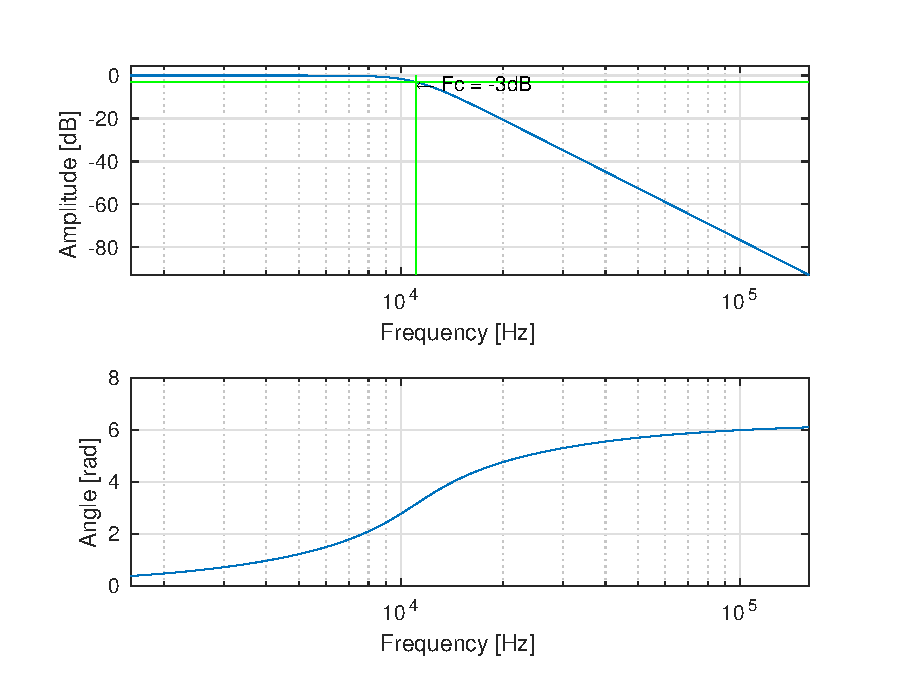
\includegraphics[width=230px]{./images/Buttcontfcny.eps}
  	\caption{Continuous low-pass filter order 4 $f_{c}=11025$ }
  	\label{contfilt}
  \end{figure}
  
\section{Using bilinear transform to produce a digital filter}
The continuous Laplace domain can't be used on numerical data,  thus it will be seen now how to convert a continuous filter to the discrete domain, referred as the $Z$ domain.\\
To pass from a domain to another the bilinear transform is used:
\begin{equation}
	s \approx \frac{2}{T_s}\frac{1-z^{-1}}{1+z^{-1}}
	\label{eq:bili}
\end{equation} 
Using the \ref{eq:bili} into the equation \ref{eq:ButterS} it's obtained:
\begin{equation}
	H_d(z)=G_0\prod_{k=1}^{n} \frac{1}{s_k+A} \space \frac{z^{-1}+1}{z^{-1} -\frac{A-s_k}{A+s_k}},
	\label{eq:numbut}
\end{equation}
where $A=\frac{2}{Ts*\omega_c}$, $Ts$ being the inverse of the sampling frequency.\\
The discrete pole $p_{zk}$ are easily recognisable:
\begin{equation}
p_{zk}=\frac{A-\frac{s_k}{\omega_c}}{A+\frac{s_k}{\omega_c}}=\frac{\frac{2}{Ts*\omega_c}-\frac{s_k}{\omega_c}}{\frac{2}{Ts*\omega_c}+\frac{s_k}{\omega_c}}.
\end{equation} 
The gain of the filter $G_z$ can also be derived from Eq. \ref{eq:numbut}:
\begin{equation}
G_z=G_0 \prod_{k=1}^{n} \frac{1}{\frac{2}{Ts*\omega_c}-\frac{s_k}{\omega_c}}.
\end{equation}
The zeros are easy to define looking at \ref{eq:numbut}, there is as much zeros equal to $-1$ than the order:
\begin{equation}
z_{zk}=-1.
\end{equation}
The Figure \ref{numlow} shows a discrete low pass filter generated using the previous method.
 \begin{figure}[h!]
 	\centering
 	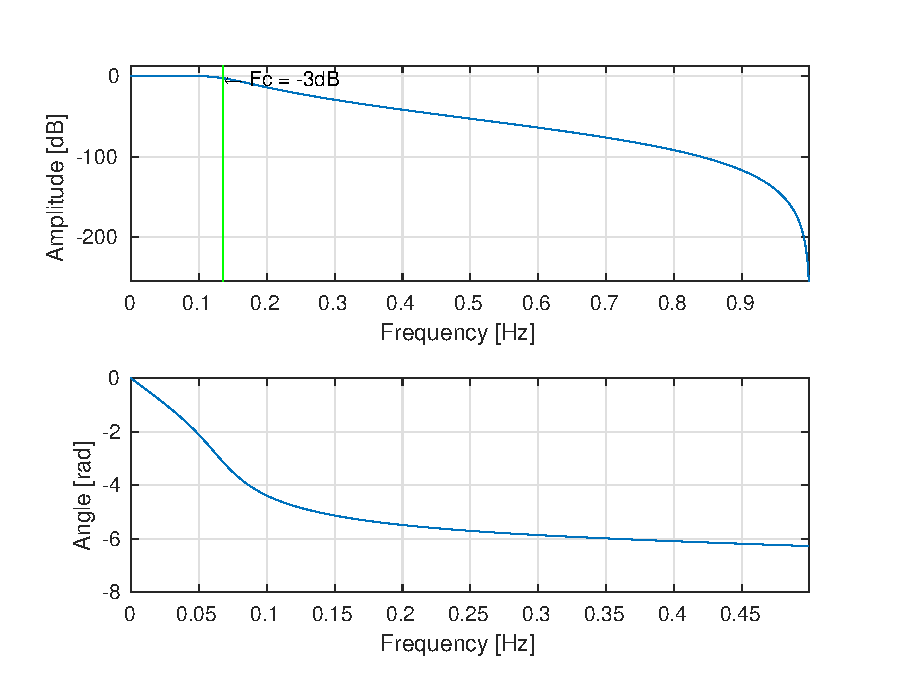
\includegraphics[width=230px]{./images/Buttnumcny.eps}
 	\caption{Discrete low pass filter order 4 $f_{c}=3000$, $f_{s}=44100\\$ }
 	\label{numlow}
 \end{figure}
  \subsection{Warping effect of bilinear transform}
  In order to determine the frequency response of the Laplace Eq. \ref{eq:ButterS}, $s$ is evaluated at $s=j\omega$, thus as the Z plane bilinear transform refers to $z=e^{sT_s}$ it means that $z=e^{j\omega T_s}$ (the form above is the first order Taylor expansion).\\
  The $z$ filter is evaluated at $H_d(z)$ while the continuous one is evaluated at $H_a(s)$, thus it's observed $e^{j\omega T_s}$ which maps $\omega$ onto $\pi F_s$.\\
  The discrete filter is mapped to $z=\omega_d =e^{j\omega T_s}$, while the continuous is mapped to $s=j\omega_a \approx\frac{2}{T}\frac{z-1}{z+1}$:
  \begin{equation}
  \begin{split}
  	H_d(z)\approx & H_a(\frac{2}{T_s}\frac{z-1}{z+1}),\\
  	H_d(e^{j\omega T_s})\approx& H_a(\frac{2}{T_s}\frac{e^{j\omega T_s}-1}{e^{j\omega T_s}+1}),\\
  	H_d(j\omega_a)\approx& H_a(j\frac{2}{T_s}tan(\frac{\omega T_s}{2})).
  	\label{eq:warpe}
  \end{split}
  \end{equation}
    This shows that the points of $H_d$ are mapped onto the continuous $s$ plane, $s=j\omega_a=e^{j\omega T_s}$. Thus, the discrete-time to continuous-time frequency mapping/warping of the bilinear transform is :
   \begin{equation}
	   \omega_a=\frac{2}{T_s}tan(\frac{\omega T_s}{2}).
   \end{equation}
   
   The warping effect of the bilinear can be compensated by setting the cut off frequency $\omega_c$ to $\frac{2}{T_s}tan(\frac{\omega_c T_s}{2})$.\\
   The warping effect is effective only in high frequency, if $\omega<<Fs/2$ then $tan(\omega)=\omega$. It's illustrated by the Figure \ref{warp}, which shows two filters at low and high frequency in both warped and unwarped case.
 \begin{figure}[h!]
 	\centering
 	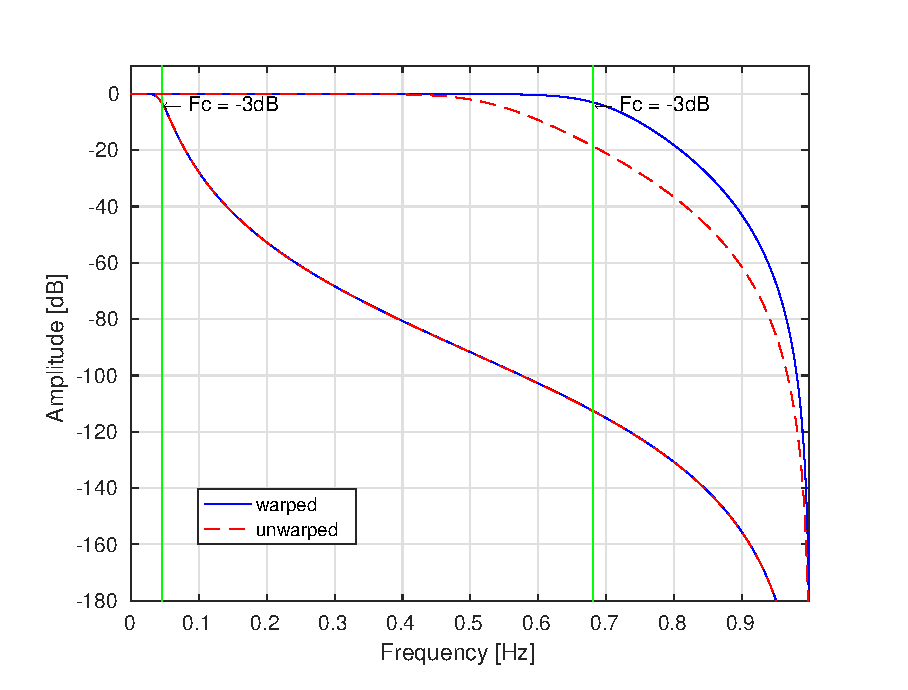
\includegraphics[width=230px]{./images/warpcomp.eps}
 	\caption{Effect of warping on two filters $f_{c}=3000Hz$, $f_{c}=15000Hz$, $F_s=44100Hz$ }
 	\label{warp}
 \end{figure}

\section{Toward a real implementation}
As the aim of the Butterworth filters is to be implemented this section will show how to implement them and some ways to reduce the calculation as well as things to pay attention.
\subsection{Precision of the variable}
Taking the  Eq.\ref{eq:polec} and Eq.\ref{eq:ButterS}  for a straight forward implementation would lead to an impossibility of calculating high order of Butterworth filter. Indeed the calculated gain would be related to $G= G_0 * (\omega_c)^n$ and would rise really fast until that there is not enough precision to calculate.\\
A simple alternative is to take into account this value at each pole modifying $s_k$ to :
\begin{equation}
s_k= e^{j\pi\frac{2k+n-1}{2n}}.
\label{eq:polemodifc}
\end{equation}
So that the pole would be written as :
\begin{equation}
p_{zk}=\frac{A-s_k}{A+s_k}=\frac{\frac{2}{Ts*\omega_c}-s_k}{\frac{2}{Ts*\omega_c}+s_k}.
\end{equation} 
The gain would be $G_z=G_0$.\\

\subsection{Pre-calculation}
If you look at the value $A$ it can be seen that to calculate the parameters of the filter you don't really need to know $F_s$ or $\omega_c$ but the ratio $\frac{Fs}{\omega_c}$. Thus this value should be calculated beforehand to reduce calculation.
\section{Using biquad implementation}
As the order of the filter is rising, the number of coefficients of the IIR filter is growing as well. This imply that the response of the filter is becoming slow, to bear with this the filter can be transformed in a cascade of second order filter, improving the speed.\\
\subsection{Biquad continuous expression}
The coefficients of these second order filters can be derived from the the analytical formulation of the continuous pole Eq.\ref{eq:polec}. A smart way to reduce the cost is to pair two poles so that the resulting second order equation as real coefficients (instead of complex ones). \\
Departing form the pole equation it can be observed for $k>1$ and $k \neq \frac{n+1}{2} \text{, for } n $ odd :
\begin{equation}
\begin{split}
s_{k} &=\overline{s_{n-k}},\\
e^{j\pi\frac{2k+n-1}{2n}} &=\overline{ e^{j\pi\frac{2(n-k)+n-1}{2n}}},\\
		&=\overline {e^{j\pi\frac{-2k+3n-1}{2n}}}=\overline {e^{j\pi\frac{-2k-n-1}{2n}}e^{j\pi\frac{4n}{2n}}},\\
		&= \overline{ e^{-j\pi\frac{2k+n-1}{2n}}*1},\\
		&=e^{j\pi\frac{2k+n-1}{2n}}.
\end{split}
\end{equation}
Thus pairing two conjugates poles ( using $s=\frac{s}{\omega_c}$) lead to:
\begin{equation}
	\begin{split}
		{(s-s_k)(s-s_{n-k})}&={s^2-s(s_k+s_{n-k})+s_ks_{n-k}},\\
		&= {s^2-s(e^{j\theta}+e^{-j\theta})+e^{j\theta}e^{-j\theta}},\\
		&= {s^2-s2cos(\theta)+1},
	\end{split}
\end{equation}
where $\theta=\pi\frac{2k+n-1}{2n}$.
It can be also observed that for odd order filter at $k=\frac{n+1}{2}$:
\begin{equation}
\begin{split}
s_{\frac{n+1}{2}}&=e^{j\pi\frac{2(\frac{n+1}{2})+n-1}{2n}},\\
 &=e^{j\pi\frac{2n}{2n}},\\
 &=e^{-j\pi}=-1.
\end{split}
\end{equation}
Using the previous statement a general formulation, known as  the normalized Butterworth polynomial $B_n$, can be written :

\begin{equation}
\begin{split}
\text{For } n \text{ even:}\\
B_n(s)&=\prod_{k=1}^{\frac{n}{2}}[s^2-2s cos(\pi\frac{2k+n-1}{2n})+1].\\ 
\text{For } n \text{ odd:}\\
B_n(s)&=(s+1)\prod_{k=1}^{\frac{n+1}{2}}[s^2-2s cos(\pi\frac{2k+n-1}{2n})+1]. 
\end{split}	
\end{equation}
The continuous expression of a low-pass filter is then expressed as:
\begin{equation}
H_a(s)=\frac{G_0}{B_n(s)}
\end{equation}
It must be kept in mind that for a desired cut off frequency $\omega_c$, the previous equation should replace $s=\frac{s}{\omega_c}$.
\subsection{Biquad digital expression}
Now that the continuous second order coefficients are known, the digital coefficients must be calculated.
Departing from the continuous second order transfer function:
\begin{equation}
H_A(s)=\frac{B_0s^2 + B_1s + B_2}{A_0s^2 + A_1s + A_2},
\label{biquadcont}
\end{equation}
and applying the bilinear transform with a warped $\omega_c$ showed before :
\begin{equation}
s=K \frac{1-z^{-1}}{1+z^{-1}},
\end{equation} 
where $K=\frac{2}{T_s*\omega_c}$, leads to the digital transfer function:
\begin{equation}
H_d(z)=\frac{b_0 + b_1z^{-1} + b_2z^{-2}}{a_0 + a_1z^{-1} + a_2z^{-2}},
\end{equation}
where the coefficients $B_i$ and $A_i$ of $H_d(z)$ calculated from $H(s)$ coefficients are :
\begin{equation}
\begin{split}
b_0&=\frac{B_0K^2+B_1K+B_2}{A_0K^2+A_1K+A_2}\\
b_1&=\frac{2B_2-2B_0K^2}{A_0K^2+A_1K+A_2}\\
b_2&=\frac{B_0K^2-B_1K+B_2}{A_0K^2+A_1K+A_2}\\
a_0&=1\\
a_1&=\frac{2A_2-2A_0K^2}{A_0K^2+A_1K+A_2}\\
a_2&=\frac{A_0K^2-A_1K+A_2}{A_0K^2+A_1K+A_2}\\
\end{split}
\end{equation} 
It can be seen that $a_0=1$ result from a normalisation of the filter, so that the original value was $a_0=A_0K^2+A_1K+A_2$.\\ \\
To go further for the optimisation, if $n>2$, it can be a good idea to normalise all the biquad filter except the first one by their respective $b_0$ so that these denominator filter coefficients will be:
\begin{equation}
\begin{split}
b_0&=1\\
b_1&=\frac{2B_2-2B_0K^2}{B_0K^2+B_1K+B_2}\\
b_2&=\frac{B_0K^2-B_1K+B_2}{B_0K^2+B_1K+B_2}\\
\end{split}
\end{equation}
A general gain should take into account each normalisation, for the number total of biquad $p$:
\begin{equation}
	G_z=\prod_{k=2}^{p}\frac{B_{p0}K^2+B_{p1}K+B_{p2}}{A_{p0}K^2+A_{p1}K+A_{p2}}.
\end{equation} 
This gain should multiply the first filter which depends if the order is odd or even :
\begin{equation}
\begin{split}
\text{For } n \text{ even:}\\
b_{1,0}&=\frac{B_0K^2+B_1K+B_2}{A_0K^2+A_1K+A_2}*G_z\\
b_{1,1}&=\frac{2B_2-2B_0K^2}{A_0K^2+A_1K+A_2}*G_z\\
b_{1,2}&=\frac{B_0K^2-B_1K+B_2}{A_0K^2+A_1K+A_2}*G_z\\
\text{For } n \text{ odd:}\\
b_{1,0}&=\frac{B_1K+B_2}{A_1K+A_2}*G_z\\
b_{1,1}&=\frac{-B_1K+B_2}{A_1K+A_2}*G_z\\
b_{1,2}&=0\\
a_{1,0}&=1\\
a_{1,1}&=\frac{-A_1K+A_2}{A_1K+A_2}\\
a_{1,2}&=0\\
\end{split}	
\end{equation} 
Finally, it can also be take into account that for low pass filter $B_0, B_1$ are null and $A_0 , A_2$ are equal to one.

\section{Other kind of filter}
\subsection{High-pass filter}
A simple way to obtain a high-pass filter using the coefficient of the low-pass is to use :
\begin{equation}
	\frac{s}{\omega_c}\rightarrow\frac{\omega_c}{s}
	\label{eq:lp2hp}
\end{equation}
Departing from the continuous transfers function:
\begin{equation}
\frac{B_0s^2 + B_1s + B_2}{A_0s^2 + A_1s + A_2}\rightarrow \frac{B_0 + B_1s + B_2s^2}{A_0 + A_1s + A_2s^2},
\label{eq:lp2hpTF}
\end{equation}
thus it's just needed to swap $B_0$ to $B_2$ and $A_0$ to $A_2$ in the previous low pass equation.\\

It obtained for all the $p$ filter expect the first one:
\begin{equation}
\begin{split}
b_{p0}&=1\\
b_{p1}&=\frac{2B_0-2B_2K^2}{B_2K^2+B_1K+B_0}\\
b_{p2}&=\frac{B_2K^2-B_1K+B_0}{B_2K^2+B_1K+B_0}\\
a_{p0}&=1\\
a_{p1}&=\frac{2A_0-2A_2K^2}{A_2K^2+A_1K+A_0}\\
a_{p2}&=\frac{A_2K^2-A_1K+A_0}{A_2K^2+A_1K+A_0}\\
\end{split}
\end{equation}
and for $p=1$:
\begin{equation}
\begin{split}
\text{For } n \text{ even:}\\
b_{1,0}&=\frac{B_2K^2+B_1K+B_0}{A_2K^2+A_1K+A_0}*G_z\\
b_{1,1}&=\frac{2B_0-2B_2K^2}{A_2K^2+A_1K+A_0}*G_z\\
b_{1,2}&=\frac{B_2K^2-B_1K+B_2}{A_2K^2+A_1K+A_0}*G_z\\
\text{For } n \text{ odd:}\\
b_{1,0}&=\frac{B_2K+B_1}{A_2K+A_1}*G_z\\
b_{1,1}&=\frac{-B_2K+B_1}{A_2K+A_1}*G_z\\
b_{1,2}&=0\\
a_{1,0}&=1\\
a_{1,1}&=\frac{-A_2K+A_1}{A_2K+A_1}\\
a_{1,2}&=0\\
\end{split}	
\end{equation}
With:
\begin{equation}
G_z=\prod_{k=2}^{p}\frac{B_{p2}K^2+B_{p1}K+B_{p0}}{A_{p2}K^2+A_{p1}K+A_{p0}}.
\end{equation} 

It's also possible to directly use the digital coefficients of the low-pass filter using the properties of the Butterworth filter. Indeed, the coefficients $A_0$ and $A_2$ are equal to 1, and the coefficient $B_0$ and $B_1$ equal to 0. Thus by observing the discrete coefficients of low pass and high pass filter it seen that the only difference is :
\begin{equation}
b_{1hp}=-b_{1lp},
\end{equation}
and 
\begin{equation}
G_{zhp}=G_{zlp}*K^n,
\end{equation}
Thus inverse the sign of $b_1$ and multiply the first filter numerator by  $K^n$.

\subsection{Bandpass filter}
A  way to obtain band pass filter using the coefficient of the low-pass is to use :
\begin{equation}
\frac{s}{\omega_c}\rightarrow\frac{\omega_c}{\Delta\omega}(\frac{s}{\omega_o}+\frac{\omega_0}{s}),
\label{eq:lp2bp}
\end{equation}
with $\omega_0=\sqrt{\omega_1\omega_2}$ and $\Delta\omega=\omega_2-\omega_1$.\\
This transformation involve a complex transformation of the filter resulting a doubled order filter (for low frequency and high frequency filtering). \\
The easiest way is to use a low pass filter combined with a high pass filter.
% The demonstration is easy if we begin by mixing Eq.\ref{eq:ButterS} and \ref{eq:lp2hp} considering one pole:
%\begin{equation}
%\begin{split}
%\frac{1}{(s/\omega_c-s_k)}& \rightarrow  \frac{s/\omega_c}{(1-s_k s/\omega_c)}.
%\end{split}
%\end{equation}
%Then using the (warped)bilinear transform:
%\begin{equation}
%\begin{split}
%\frac{K \frac{1-z^{-1}}{1+z^{-1}}}{(1-s_kK \frac{1-z^{-1}}{1+z^{-1}})}&=\frac{K (1-z^{-1})}{(1+z^{-1}-s_kK( 1-z^{-1})}\\
%& =\frac{K (1-z^{-1})}{z^{-1}(1+Ks_k) +(1-Ks_k)}\\
%& =\frac{K}{(1+Ks_k)}\frac{ (1-z^{-1})}{z^{-1} +\frac{(1-Ks_k)}{(1+Ks_k)}}\\
%\end{split}
%\end{equation}

%\section{Conclusion}



\begin{thebibliography}{99} % Bibliography - this is intentionally simple in this template
\bibitem[\href{https://www.mathworks.com/help/signal/ref/bilinear.html}{https://www.mathworks.com/help/signal/ref/bilinear.html}]{site1}
\bibitem[\href{https://en.wikipedia.org/wiki/Bilinear\_transform}{https://en.wikipedia.org/wiki/Bilinear\_transform}]{site2}
\bibitem[\href{https://en.wikipedia.org/wiki/Butterworth\_filter}{https://en.wikipedia.org/wiki/Butterworth\_filter}]{site3}

%\newblock Assortative pairing and life history strategy - a cross-cultural
%  study.
%\newblock {\em Human Nature}, 20:317--330.
 
\end{thebibliography}--------------------------------------------------

\newpage
\appendix

\section{Bilinear demo Eq. \ref{eq:numbut}}
\begin{equation*}
\begin{split}
\frac{1}{\frac{w_c}{s-s_k}}
\rightarrow\frac{1}{\frac{A(1-z^{-1})}{1+z^{-1}}-\frac{s_k}{\omega_c}} 
=\frac{z^{-1}+1}{B-Bz^{-1}-\frac{s_k}{\omega_c}-z^{-1}\frac{s_k}{\omega_c}}\\
=\frac{z^{-1}+1}{z^{-1}(-\frac{s_k}{\omega_c}-B)-B-\frac{s_k}{\omega_c}}
\end{split}
\end{equation*}
\section{Warping demo Eq. \ref{eq:warpe}}
\begin{equation*}
\begin{split}
\frac{e^{j\omega T_s}-1}{e^{j\omega T_s}+1} &= \frac{e^{j\omega T_s/2}(e^{j\omega T_s/2}-e^{j\omega T_s/2})}{e^{j\omega T_s/2}(e^{j\omega T_s/2}+e^{j\omega T_s/2})}\\
& = \frac{j(e^{j\omega T_s/2}-e^{j\omega T_s/2})/2j}{(e^{j\omega T_s/2}+e^{j\omega T_s/2})/2}\\
&  =j \frac{sin(\omega T_s/2)}{cos(\omega T_s/2)}\\
& = jtan(\frac{\omega  T_s}{2})
\end{split}
\end{equation*}

%----------------------------------------------------------------------------------------

\end{document}
